\documentclass[12pt]{article}
\usepackage[utf8]{inputenc}
\usepackage{url}
\usepackage{hyperref}
\usepackage{amsmath}
\usepackage[usenames,dvipsnames]{color}
\usepackage{graphicx}
% Colors
\definecolor{olincolor}{rgb}{0.13,0,0.7}
\hypersetup{
linkcolor=olincolor,
citecolor=olincolor,
urlcolor=olincolor,
anchorcolor=olincolor,
filecolor=olincolor,
colorlinks=true
}
\usepackage{float}
\usepackage{soul}


\newtheorem{ex}{Exercise}


\title{Simulating Virtual Creatures}
\date{}
\begin{document}
  \maketitle 
\newcommand{\TODO}{\hl{\emph{TODO:}}\hl}

In 1994, a researcher named Karl Sims simulated Darwinian evolution using virtual block creatures interacting with each other in a virtual environment.  His work spawned creatures both familiar and alien to those we find on our planet: \url{http://www.youtube.com/watch?v=JBgG_VSP7f8}. 

Much of what computer scientists do is deterministic and heavily controlled. However, like Conway’s Game of Life, genetic algorithms can produce behavior we would never have imagined. Utilizing unexpected behavior can be a critical tool in exploring a solution space that may be too vast or computationally too expensive to define. Given enough time and the right set of evolutionary mechanisms, a genetic algorithm can find solutions to ungainly problems, just as Darwinian evolution has bred significant complexity and efficiency into living organisms over billions of years.


\section{Artificial Neural Networks}

How do brains work? At the most basic level, a brain is a small world network that takes in sensory input from the environment (visual, auditory, tactile, etc...) an produces some output, often in the form of muscle movement. The basic units of computation are neurons, which roughly cdorrespond to the logic gates of a CPU. Consequently, brains are known as \emph{neural networks} (NNs). For decades, computer scientists have been creating artificial representations of these biological systems in an attempt to simulate human thought in computers. Despite repeated failures in this holy grail of artificial intelligence (AI) research, NNs have successfully been used to perform non-linear data analysis in fields such as pattern matching, image recognition, and game AIs.

While logic gates in processors only deal with binary values, nodes in most NNs support real numbers.\footnote{Nevertheless, some neuron implementations deal with integers, binary values, or a mix of types} As shown below, every neuron in a network evaluates a function that operates on one or more inputs to produce one or more output values. Each edge in the graph has a weight associated with it, which scales the value passed in:

\begin{figure}[H]
\centerline{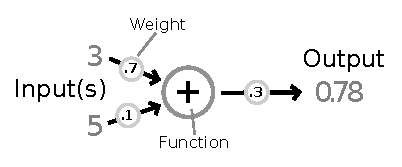
\includegraphics[height=1.5in]{figs/Neuron}}
\end{figure}



In this example of a sum node, the input values \verb|(3,5)| yield an 0.78 as the output: $(0.7\times 3)+(0.1\times 5) \Rightarrow 2.6$; $2.6 \times 0.3 \Rightarrow 0.78$. The weights generally start out random and are updated until the NN "learns" how to produce appropriate outputs. The function of a given neuron could be any operation on a set of numbers, including (but not limited to) difference, product, and sine. More complicated nodes can have a memory component.

The simplest type of NN is known as a \emph{feed forward} network, which is a directed graph with \emph{hidden} computation layers that act on the values of several input nodes and yield values for one or more output nodes:

\begin{figure}[H]
\centerline{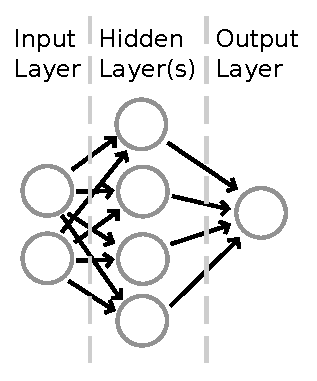
\includegraphics[height=2.5in]{figs/NN}}
\end{figure}
\emph{Training} is the process of adjusting a neural network to solve problems by adjusting the weights present in the network. The weights in this type of NN are often modified over time using the \emph{backpropagation} training algorithm, which you can read about here: \url{http://en.wikipedia.org/wiki/Back_propagation.}

NNs like this are ideal for problems with answers are not clear cut, such as handwriting recognition. A NN could be trained to take in a (simplified) image and output a letter and how confident it is in that answer.

More complicated NNs can contain cycles and have no clear separation between the layers of the network:

\begin{figure}[H]
\centerline{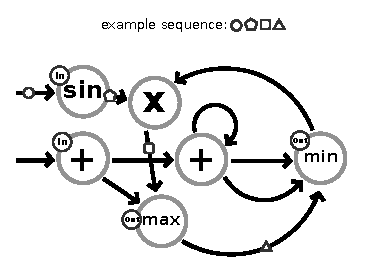
\includegraphics[height=2.5in]{figs/ComplexNN}}
\end{figure}
In this example, we follow a sequence of four data elements as they travel through the network (obviously, the values change every time they move between nodes, but this isn't shown in the diagram). Note that the weights of the edges aren't shown and that the second input node's data stream would move in sync with the stream that is depicted above. Depending on the implementation of the network, edges that have never encountered data before are ignored or assigned a value of zero when they propagate data to the nodes.


\begin{ex}
Read more about NNs here: \url{http://en.wikipedia.org/wiki/Artificial_neural_network}.
 What learning paradigm does back-propagation fall into?
\end{ex}

\begin{ex}
Implement your own feed forward neural network using nothing but sum nodes. Can you train it to approximate the sine function? You can download our solution \TODO{HERE}.
\end{ex}

\section{Genetic Algorithms}

Like NNs, genetic algorithms are based on real biological behaviors. They are used to solve problems by breeding the \emph{fittest} of several potential solutions in the hope of finding even better solutions, which makes them analogous to the process of Darwinian Evolution. Genetic algorithms are a subset of \emph{Evolutionary Algorithms}, which you can read about here: \url{http://en.wikipedia.org/wiki/Evolutionary_algorithm}.

The basic process of a genetic algorithm has the following five steps:

\begin{enumerate}
\item Generate an initial \emph{population} of potential solutions. These initial solutions are usually random.

\item Evaluate the "goodness" of each \emph{individual} in the population using a \emph{fitness} function.

\item Select $n$ individuals such that high fitness individuals are more likely to be selected.

\item Breed these individuals by combining traits of the existing individuals and \emph{mutating} some of these traits randomly. Breeding methods depend on implementation, but they can include asexual cloning, asexual mutation and crossover. This results in a new generation (usually constrained to have the same number of individuals as the previous generation).

\item Repeat steps 2-5 with each new generation.
\end{enumerate}
How do genetic algorithms solve problems? All possible solutions to a problem exist within a \emph{solution space} and a genetic algorithm is a type of \emph{search algorithm} for finding the optimal solution in that space.

\begin{figure}[H]
\centerline{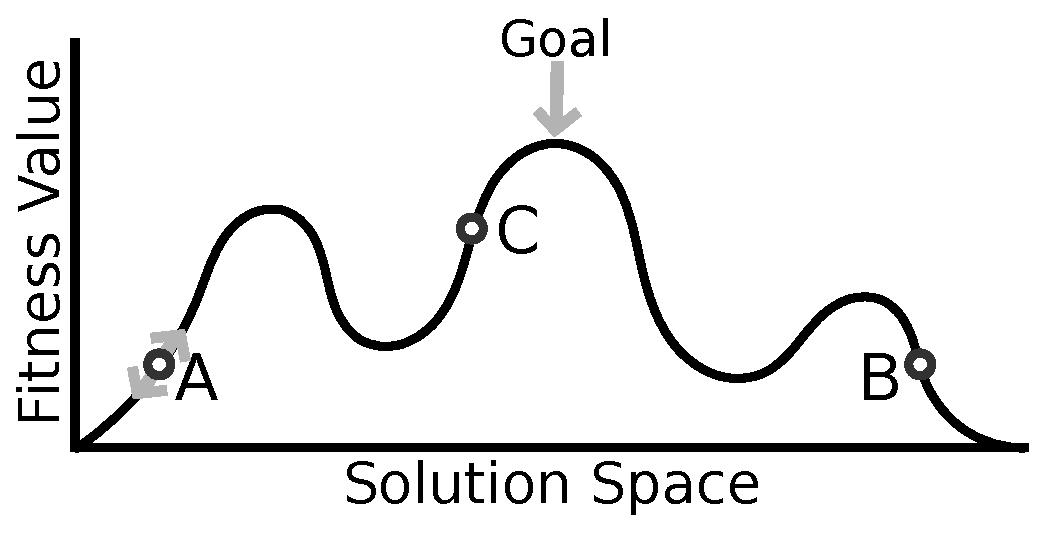
\includegraphics[height=2in]{figs/GeneticAlgStateSpace}}
\end{figure}

In the diagram above, \verb|A| and \verb|B| represent randomly generated individuals with relatively low fitness values. During breeding, there is a chance that a trait is mutated. This usually results in a lower fitness value, but can at times be beneficial, as the arrows around A indicate.\footnote{Depending on the trait being mutated and the degree of mutation, it is also possible that the resulting solution could lie on a different hill in the solution space.} Breeding between two individuals generally involves a \emph{crossover} of traits between those individuals, with the goal of mixing good behaviors in order to create a new individual on a different hill in the solution space. For example, breeding \verb|A| and \verb|B| could result in \verb|C| in the diagram above, which is closer to the global maximum than either of its parents.
 
\begin{ex}
Read more about genetic algorithms on wikipedia: \url{http://en.wikipedia.org/wiki/Genetic_algorithm}. List several ways that individuals in the population could be represented.
\end{ex}

\begin{ex} Eight Queens
Eight Queens is a classic puzzle that asks how eight queens can be placed on an 8-by-8 chessboard such that no two queens can attack each other (i.e. no two queens share the same column, row, or diagonal). Since there are $8 \times 8 = 64$ squares in the chessboard, there are ${64 \choose 8} = 4426165368$ possible arrangements of the eight queens. 

Finding one of the 92 solutions in this large space by brute force is highly inefficient. Instead, we’ll break out a genetic algorithm. Our individual is a particular arrangement of the queens, stored as a list of eight \verb|(row, column)| tuples:

\begin{verbatim}
import genetics
class Arrangement(genetics.Individual):
	“””Represents a particular arrangement of 8 queens.”””
	
	def __init__(self, queens=None):
		“””Create a new arrangement of queens.

		If queens is given, then use that list of positions, otherwise
		initialize to a random arrangement.
		“””
		genetics.Individual.__init__(self)
		self.queens = queens or self.makeRandomQueens()
\end{verbatim}

To create a random arrangement and allow for mutations, we’ll use the \verb|mutations| module:
\begin{verbatim}
import mutations
...
# row is an integer between 1 and 8, which mutates 5% of the time.
randomRowValue = mutations.MutableInt((1, 8), rate=0.05)
# column is an integer between 1 and 8, which mutates 5% of the time.
randomColumnValue = mutations.MutableInt((1, 8), rate=0.05)

def makeRandomQueens(self):
	“””Return a list 8 random (row, column) queen positions.”””
	def makeRandomQueen():
		return self.randomRowValue(), self.randomColumnValue()
	return [makeRandomQueen() for _ in range(8)]

def mutate(self):
	“””Returns a mutated version of this arrangement.”””
	
	# Calling self.randomRowValue with row either returns the same value
	# or 5% of the time, mutates the value to a nearby row chosen at random.
	# Same for self.randomColumnValue
	newQueens = [(self.randomRowValue(row), self.randomColumnValue(col))
                   for row, col in self.queens]
	return Arrangement(newQueens)
\end{verbatim}

Finally, we need a way to \emph{crossover} parts of two different arrangements:
\begin{verbatim}
import random
...
def crossover(self, otherArrangement):
	crossoverPoint = random.randint(0, 8-1)
	newQueens = self.queens[:crossoverPoint] + \
otherArrangement.queens[crossoverPoint:]
	return Arrangement(newQueens)
\end{verbatim}

\TODO{Will finish eight queens example to explain the rest of the framework}

\end{ex}

\section{Implementing Neural Networks and Genetic Algorithms}

Using NetworkX and directed graphs to do this


\section{Making Virtual Creatures}

\subsection{Representing Creatures}
As is standard in genetic algorithms, creatures are referred to as individuals. Individuals have two fundamental components: a brain and a body. 

\subsubsection{The body}
We define the body of a creature using a Morphology object. This object wraps a MultiDirectedGraph \TODO{(we should talk about why we use a multidirected graph, and perhaps how/why we expand it into a Tree)}.  In this graph, each body part is represented as a node, and connections between body parts are represented as edges. The directed graph allows cycles, and thus when building a physical representation, the expand() method is used to create a tree that is easy to parse, in this process a recursion limit is imposed. An example morphology and the body defined by the morphology is provided below:\TODO{this needs to be fleshed out and rewritten}

\subsubsection{The mind}
The brain of a creature is represented as a neural network as detailed previously.  The outputs of the neural network are mapped to actuators located in the joint between two body parts. \TODO{link this to body}

\subsection{Simulating Creatures in Physical Environments}
The physics package \verb|PyBox2d| is well suited for physics implementation and calculations, it provides joints, rigid bodies and collision detection. In order to visualize the creatures, we use a popular visualization library, \verb|PyGame|. Abstracting further away from the details of physics implementation, a Simulation Environment object was created to encapsulate the world in which virtual creatures are simulated, it provides physics simulation and visualization.
Here is a simple example program to create a simple creature and simulate it.
\begin{verbatim}
from critters.physics import simulationEnvironment
from critters.physics import objects
from critters import neural, life, morph
import random
\end{verbatim}

First create an empty Morphology
\begin{verbatim}
iWorm = morph.Morphology() #instantiate an `empty' morphology
\end{verbatim}

Add two body parts to the morphology  as follows:
\begin{verbatim}
head = morph.MorphNode(dimensions=(2,2)) #create a node representing the head
tail = morph.MorphNode(dimensions=(2,2)) #create a node representing the tail
\end{verbatim}

Create random locations on the two bodies to create a connection between
\begin{verbatim}
conLocations=(random.randint(0,4),random.randint(0,4))#select random vertices
\end{verbatim}
Add a connection between the two body parts, located at \verb|conLocations|, an integer representing the local location
\begin{verbatim} 
iWorm.addConnection(morph.MorphConnection((head,tail),locations=conLocations))
\end{verbatim}
Create a simple neural network made of sine nodes to act as the brain of this simple creature
\begin{verbatim}
net = neural.simpleSineNetwork(1, 1) #create a simple neural network
\end{verbatim}
Combine the morphology and the neural network and create a creature to encapsulate these two ideas:
\begin{verbatim}
creature = life.Critter(numSensors=1,morphology=iWorm, neuralNet=net)
\end{verbatim}
Create a simulation environment and add the creature to it:
\begin{verbatim}
simEnv = simulationEnvironment.SimulationEnvironment()
simEnv.addCreature(creature)
\end{verbatim}
Then simply ask the simulation environment to simulate, the optional parameter of timeToRun is set to None to run infinitely.
\begin{verbatim}
simEnv.simulate(offset=(500,-300),timetoRun = None) #offset is for initial window placement
\end{verbatim}

\begin{ex}
If you're feeling adventurous, try to port our implementation of Karl Sims' work to 3D. To get you started, you should look into PyODE (http://pyode.sourceforge.net/) or PyBullet (https://launchpad.net/pybullet) for physics engines and PyOpenGL (http://pyopengl.sourceforge.net/) or VPython (http://vpython.org/) for visualization.
\end{ex}

\end{document}